\documentclass[11pt,spanish,a4paper]{article}
\usepackage[utf8]{inputenc}                         % UNICODE
\usepackage[T1]{fontenc}                            % Permite copiar caractéres unicode desde el PDF al portapapeles
\usepackage{amsmath}                                % Matemáticas American Mathematical Society
\usepackage{amssymb}                                % Math symbols
\usepackage{graphicx}                               % Insertar gráficos
\usepackage[ddmmyyyy]{datetime}                     %
\usepackage[spanish, es-nodecimaldot]{babel}        % Corte de las palabras en español
\usepackage{enumitem}
\usepackage[hidelinks]{hyperref}                    % Enlaces sin apariencia fea
\usepackage{siunitx} \sisetup{ output-decimal-marker={,}, quotient-mode=fraction}   % Sistema internacional para unidades con separador decimal
\usepackage{gensymb}                                % Símbolos de grado
\usepackage{geometry}                               % Cambiar márgenes del documento
\usepackage[pscoord]{eso-pic}                       % Overlay text. The zero point of the coordinate system is the lower left corner of the page (the default).
\usepackage{titlesec}								% Change title of section and subsection
\usepackage{fontspec}								% Use other font
\usepackage{xcolor}
\usepackage[]{minted}
\renewcommand{\listingscaption}{Listado}

%\newgeometry{top=15mm, bottom=20mm, left=15mm, right=15mm}

% Color =======================
\definecolor{azul}{RGB}{0,106,255}
\definecolor{bg}{rgb}{0.95,0.95,0.95}

% Cambio subsección ==========================================
\titleformat{\section}
  {\Large\bfseries}  						% The style of the section title
  {\color{azul}Proyecto \thesection}    	% a prefix
  {20pt}                         			% How much space exists between the prefix and the title
  {\color{azul}}    						% How the section is represented
% Fuente ==================================
\setmainfont{Atkinson-Hyperlegible-Regular-102.otf}[
	Path = font/,
	BoldFont = Atkinson-Hyperlegible-Bold-102.otf,
	ItalicFont = Atkinson-Hyperlegible-Italic-102.otf,
	BoldItalicFont = Atkinson-Hyperlegible-BoldItalic-102.otf]

\title{Proyectos para Tecnología, Programación y Robótica}
\author{Samuel Gómez}

\begin{document}

\maketitle
\vspace{2cm}
\begin{center}

\includegraphics[height=6cm]{img/arduino_logo.jpg}
\end{center}

\newpage
\tableofcontents
% PROYECTOS PARA PRÁCTICAR
% Proyecto 0.1 ----------------------------
\newpage
\section{Hola mundo}

\subsection{Objetivos}
Este proyecto sirve para testear un LED y empezar a familiarizarse con la
placa de pruebas.

\subsection{Pasos para desarrollar el proyecto}
\begin{enumerate}
	\item Colocar la placa Arduino a la izquierda y la placa de pruebas a la derecha
	\item Buscar en el LED el ánodo y el cátodo y luego colocarlo en la placa de pruebas
	\item Realizar el cableado siguiendo el esquema
	\item Escribir el software en el editor Arduino y subirlo para probarlo
\end{enumerate}

\begin{center}
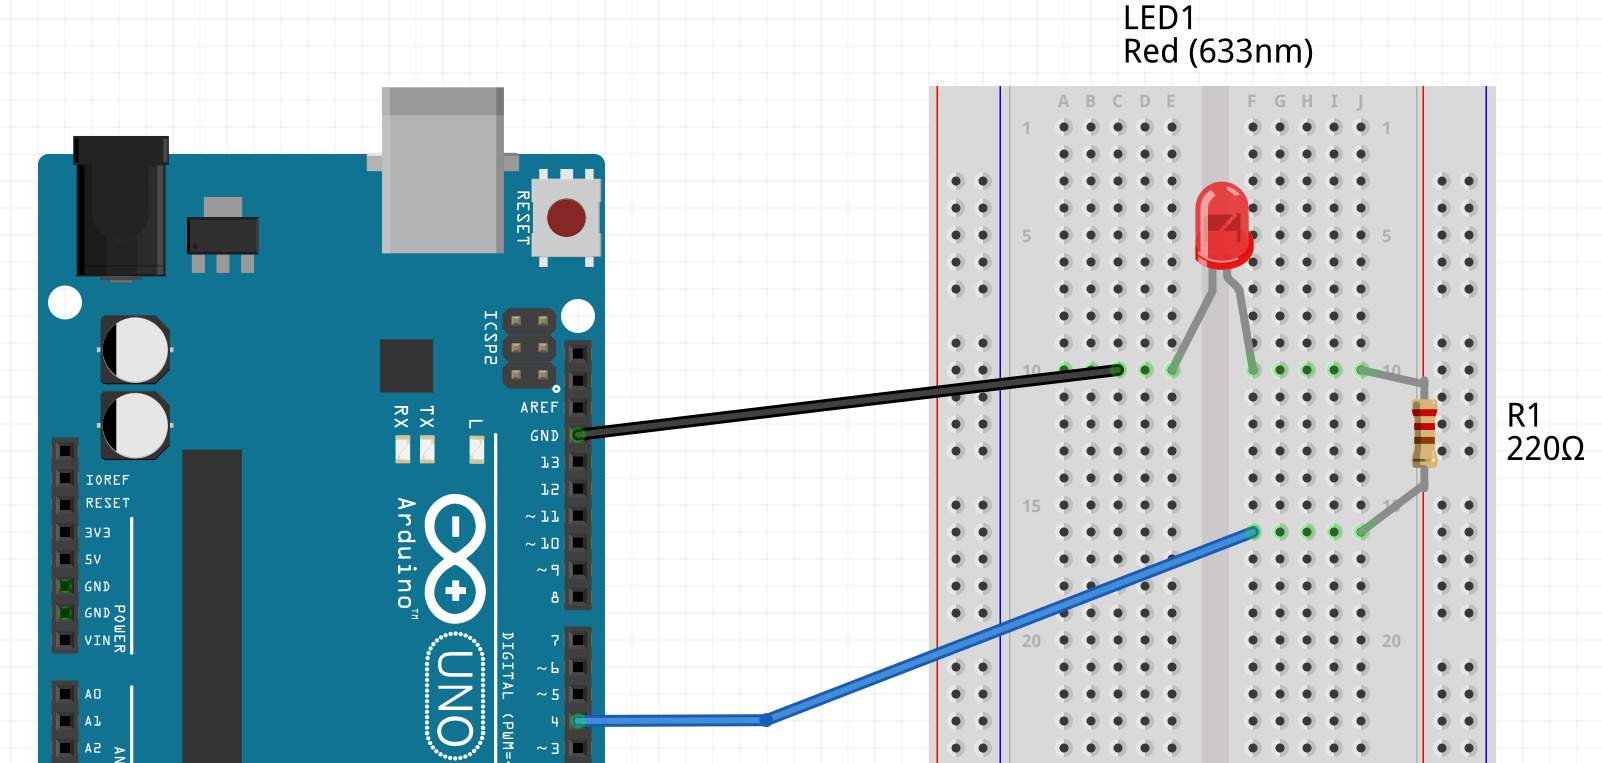
\includegraphics[height=6cm]{img/01.jpg}
\end{center}

\begin{listing}[H]
\begin{minted}[linenos=true,bgcolor=bg]{c++}
void setup() {
    pinMode(4, OUTPUT);
}

void loop() {
    digitalWrite(4, HIGH);
    delay(1000);
    digitalWrite(4, LOW);
    delay(1000);
}
\end{minted}
\caption{Software del proyecto \thesection}
\end{listing}


% Proyecto 0.2 ---------------------------
\newpage
\section{Botón doble LED}

\subsection{Objetivos}

Este proyecto sirve para prácticar la conexión de un botón y de un LED.

\subsection{Pasos para desarrollar el proyecto}
\begin{enumerate}
	\item Montar el botón siguiendo el esquema
	\item Montar el LED de color rojo y conectarlo al puerto 4
	\item Montar el LED de color verde y conectarlo al puerto 5
	\item Escribir el software y probarlo y conectarlo al puerto 6
\end{enumerate}

\begin{center}
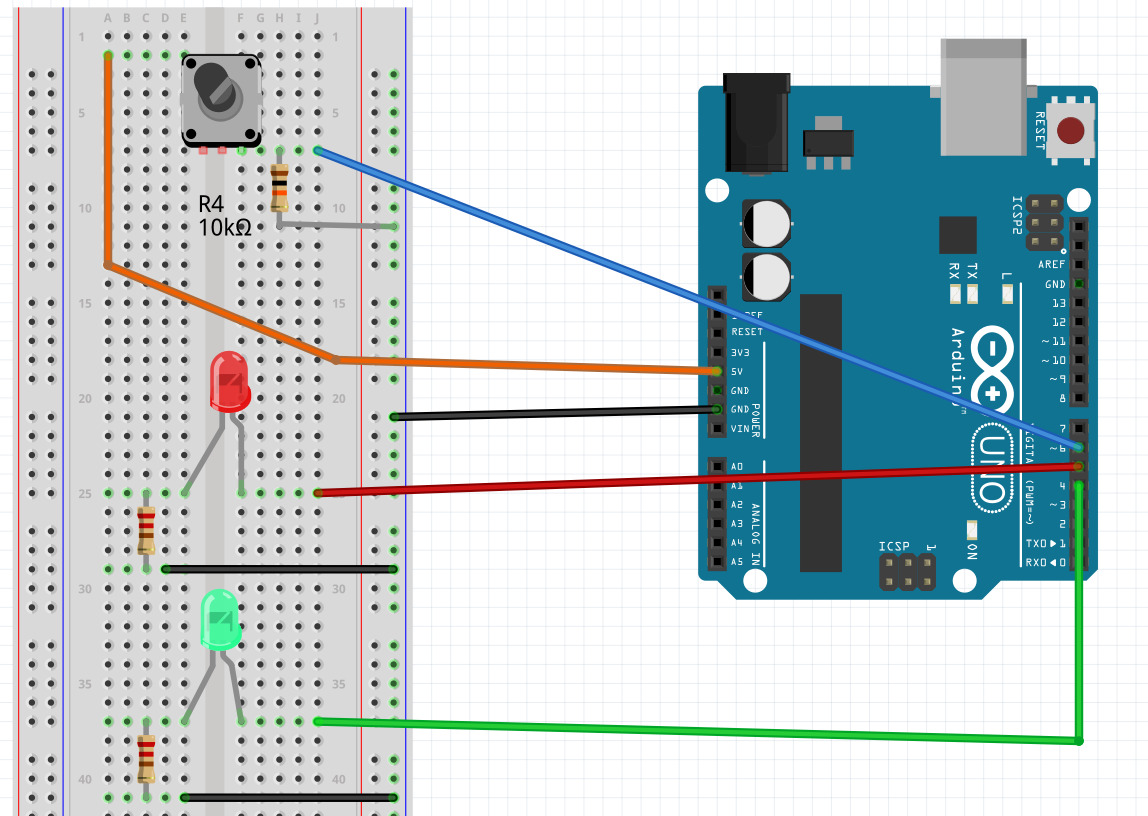
\includegraphics[height=6cm]{img/02.jpg}
\end{center}

\begin{listing}[H]
\begin{minted}[linenos=true,bgcolor=bg]{c++}
void setup() {
    pinMode(4, OUTPUT);
    pinMode(5, OUTPUT);
    pinMode(6, INPUT);
}

void loop() {
    if (digitalRead(6)==HIGH){
        digitalWrite(4, HIGH);
        digitalWrite(5, LOW);
    } else {
        digitalWrite(4, LOW);
        digitalWrite(5, HIGH);
    }
}
\end{minted}
\caption{Software del proyecto \thesection}
\end{listing}


% ------------------------------------------------
% Proyecto 0.3
\newpage
\section{Semáforo de tres luces}

\subsection{Objetivos} Las luces se encenderán siguiendo el orden

\subsection{Pasos para desarrollar el proyecto}
\begin{enumerate}
	\item El LED rojo se conecta al puerto 4
	\item El LED ambar se conecta al puerto 5
	\item El LED verde se conecta al puerto 6
	\item La luz roja luce durante 7 segundos, luego la verde 7 y finalmente la ambar durante 1
		segundo antes de volver a comenzar el ciclo
\end{enumerate}

\begin{center}
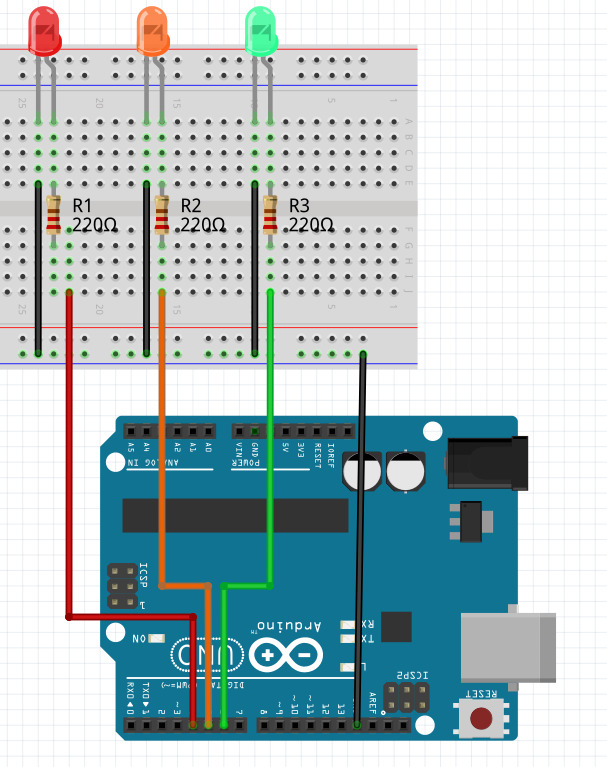
\includegraphics[height=11cm]{img/03.jpg}
\end{center}

\begin{listing}[H]
\begin{minted}[linenos=true,bgcolor=bg,autogobble]{c++}
void setup() {
    pinMode(4, OUTPUT);
    pinMode(5, OUTPUT);
    pinMode(6, OUTPUT);
}

void loop() {
    digitalWrite(4,HIGH);
    digitalWrite(5,LOW);
    digitalWrite(6,LOW);
    delay(7000);

    digitalWrite(4,LOW);
    digitalWrite(5,LOW);
    digitalWrite(6,HIGH);
    delay(7000);

    digitalWrite(4,LOW);
    digitalWrite(5,HIGH);
    digitalWrite(6,LOW);
    delay(1000);
}
\end{minted}
\caption{Software del proyecto \thesection}
\end{listing}


% ------------------------------------------------
% Proyecto 0.4
\newpage
\section{Piezoeléctrico, LED y botón}

\subsection{Objetivos} El piezoeléctrico emitirá pitidos a intervalos de un segundo, y una frecuencia
de 3000 Hz. El LED rojo
parpadeará cuando suene el pitido. El botón inhibe el sonido del piezo, pero no del LED.

\subsection{Pasos para desarrollar el proyecto}
\begin{enumerate}
	\item El piezoeléctrico se conecta al puerto 9
	\item El LED rojo se conecta al puerto 4
	\item El botón se conecta al puerto 5
	\item Cuando el botón se pulsa, el sonido no se inhibe sino que suena otro tono diferente
\end{enumerate}

\begin{center}
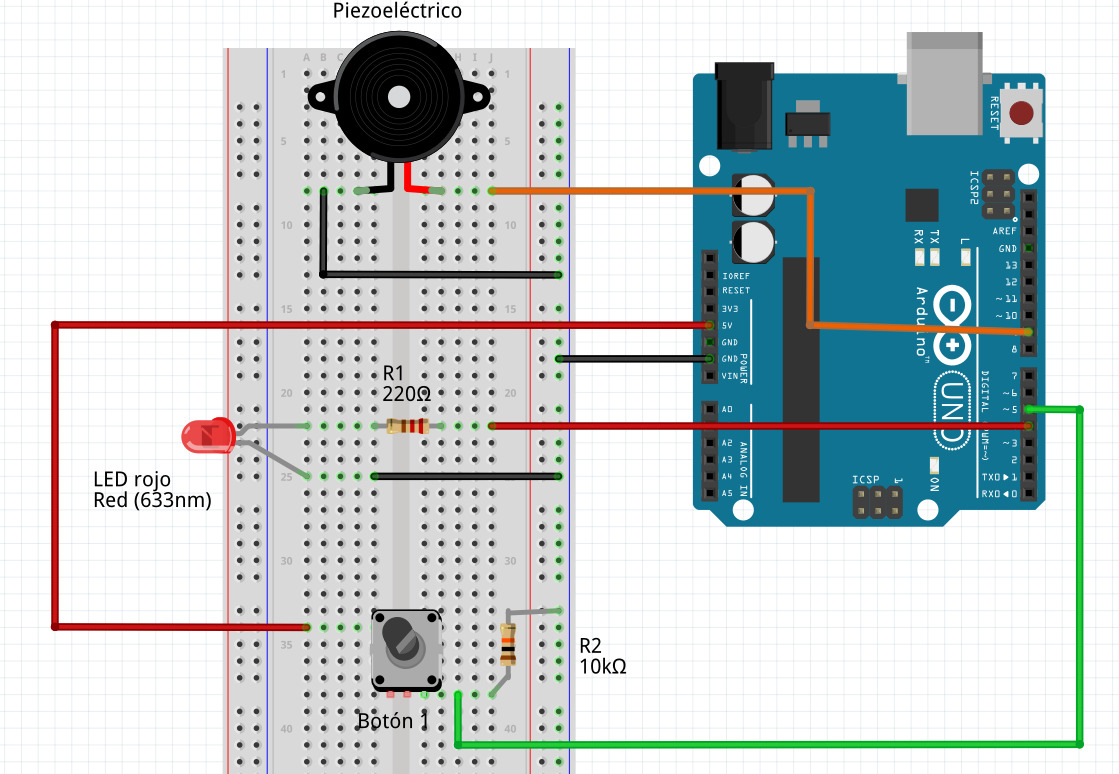
\includegraphics[height=12cm]{img/04.jpg}
\end{center}

\begin{listing}[H]
\begin{minted}[linenos=true,bgcolor=bg,autogobble]{c++}
void setup() {
    pinMode(4, OUTPUT);
    pinMode(5, OUTPUT);
    pinMode(6, INPUT);
}

void loop() {
    if (digitalRead(6)==HIGH){
        digitalWrite(4, HIGH);
        digitalWrite(5, LOW);
    } else {
        digitalWrite(4, LOW);
        digitalWrite(5, HIGH);
    }
}
\end{minted}
\caption{Software del proyecto \thesection}
\end{listing}


% ------------------------------------------------
% Proyecto 0.5
\newpage
\section{Emisor de código morse}

\subsection{Objetivos} En este proyecto construimos una máquina generadora de código morse con dos
botones. El código morse se empleaba en transmisiones telegráficas y cada letra tiene su
representación. En nuestro hardware, dos botones controlan los pitidos del piezoeléctrico. Uno produce pitidos
cortos y otro produce pitidos largos.

\subsection{Práctica} Prueba a emitir un mensaje de SOS, para ello comprueba en la Figura 
\ref{cod_morse} a que conjunto de puntos y letras corresponde cada letra (S, O, S).

\begin{figure}[H]
\centering
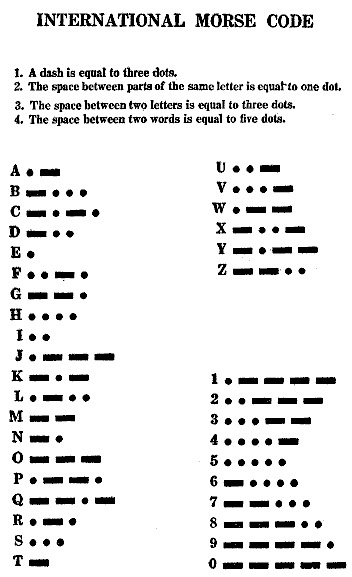
\includegraphics[width=6cm]{img/05.02.jpg}
\caption{Código Morse}
\label{cod_morse}
\end{figure}

\subsection*{Pasos para desarrollar el proyecto}
\begin{enumerate}
	\item Se desarrolla y se sube el software
	\item El piezoeléctrico se conecta al puerto 9
	\item El botón $A$ se conecta al puerto 4
	\item El botón $B$ se conecta al puerto 5
\end{enumerate}

\begin{center}
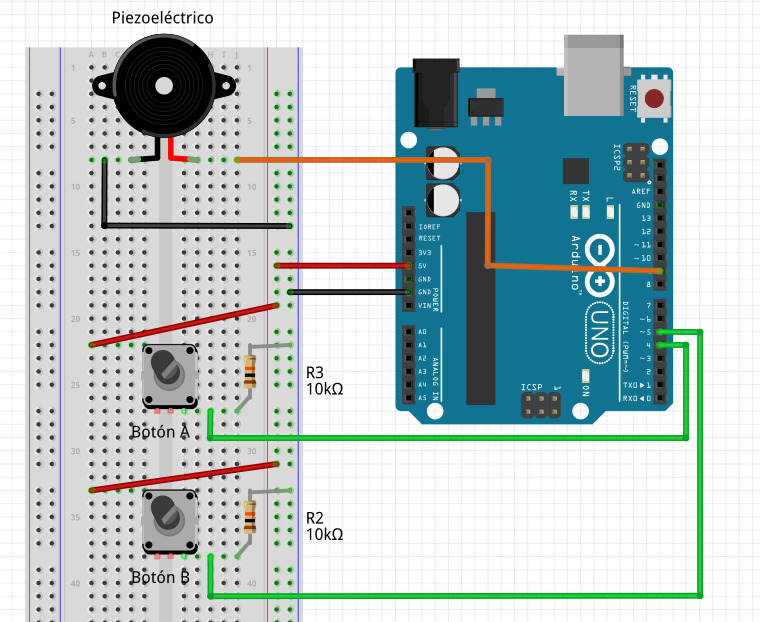
\includegraphics[width=12cm]{img/05.jpg}
\end{center}

\begin{listing}[H]
\begin{minted}[linenos=true,bgcolor=bg,autogobble]{c++}
void setup() {
  pinMode(4, INPUT);
  pinMode(5, INPUT);
  pinMode(9, OUTPUT);
}

void loop() {
  if (digitalRead(4)==HIGH){  // Si se pulsa el botón 4
    tone(9, 3000, 100);
  }
  if (digitalRead(5)==HIGH){  // Si se pulsa del botón 5
    tone(9, 3000, 300);
  }
  delay(500);
}
\end{minted}
	\caption{Software del proyecto \thesection}
\end{listing}


% -----------------------------------------------------
% PROYECTOS PARA EVALUAR
% -----------------------------------------------------
\newpage
\section{Botón de control}
\subsection{Pasos para desarrollar el proyecto}
\begin{enumerate}
	\item Montar un LED rojo en el puerto 5 y uno verde en el 6 (HW)
	\item El LED rojo debe parpadear a intervalos de 1 segundo (SW)
	\item Montar un botón en el puerto 3 (HW)
	\item Si se pulsa el botón, el LED verde debe encenderse (SW)
\end{enumerate}

\section{Alarma}
\subsection*{Pasos para desarrollar el proyecto}
\begin{enumerate}
	\item Poner un piezoeléctrico conectado al puerto 9 (HW)
	\item El piezoeléctrico debe emitir un pitido cada segundo (SW)
	\item Montar un LED rojo conectado al puerto 7 (HW)
	\item El LED rojo debe parpadear intermitentemente cuando suene la alarma (SW)
\end{enumerate}


\section{Semáforo con aviso acústico}

\textbf{Nota} Este proyecto presenta una dificultad añadida ya que el software del paso 2 y el 3
son diferentes. Además, el paso 4 depende tanto de hardware como de software para poder ser
completado.

\subsection{Pasos para desarrollar el proyecto}
\begin{enumerate}
	\item Montar un LED verde y otro rojo en los puertos 4 y 5 respectívamente (HW)
	\item Los LED deben encenderse secuencialmente a intervalos de 4 segundos (SW)
	\item El LED verde debe estar encendido 2 segundos, luego parpadea a intervalos de medio segundo
		(durante dos segundos) antes de cambiar al rojo (SW)
	\item Conectar un piezoeléctrico al puerto 6 y hacer que emita un pitido cuando el semáforo esté
		en verde (HW + SW)
\end{enumerate}

% ----------------------------------------------------
\section{Monitor serie}

\subsection{Objetivos}
\textbf{Este proyecto no se firma} Este es un proyecto que servirá para realizar pruebas.

\subsection{Primer software}

\begin{listing}[H]
\begin{minted}[linenos=true,bgcolor=bg,autogobble]{c++}
void setup() {
  Serial.begin(9600);
}

void loop() {
  Serial.println("Hola");
}
\end{minted}
	\caption{Primer software del proyecto \thesection}
\end{listing}

\subsection{Segundo software}

\begin{listing}[H]
\begin{minted}[linenos=true,bgcolor=bg,autogobble]{c++}
int n = 0;              // Inicializa la variable

void setup() {
  Serial.begin(9600); // Inicializa monitor serie
}

void loop() {
  n++;                // Incrementa la variable 
  Serial.println(n);  // Mostrar en pantalla el valor
  delay(100);
}
\end{minted}
	\caption{Segundo software del proyecto \thesection}
\end{listing}



\newpage
%--------------------------------------------------------------------------
\section{Servomotor}

\subsection{Objetivos}

\textbf{Este proyecto no se firma} Este es un proyecto que servirá para realizar pruebas.

\begin{center}
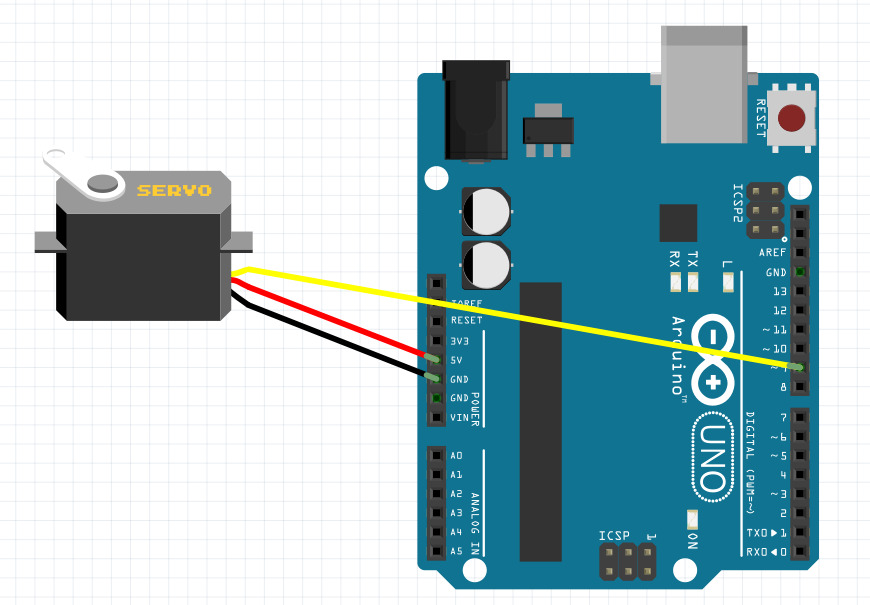
\includegraphics[height=5cm]{img/06.jpg}
\end{center}

\subsection{Primer software}

\begin{listing}[H]
\begin{minted}[linenos=true,bgcolor=bg,autogobble]{c++}
#include <Servo.h>

Servo s1;             // Asigna nombre al servo

void setup() {
  s1.attach(9);       // Conectado al puerto 9
}

void loop() {
  s1.write(0);        // Posición 0 grados
  delay(1000);
  s1.write(90);       // Posición 90 grados
  delay(1000);
}
\end{minted}
\caption{Primer software del proyecto \thesection}
\end{listing}

\subsection{Segundo software}

\begin{listing}[H]
\begin{minted}[linenos=true,bgcolor=bg,autogobble]{c++}
#include <Servo.h>

Servo s1;
int p = 0;             // posición

void setup() {
  s1.attach(9);
}

void loop() {
  p++;                 // Incrementa p
  s1.write(p);         // Mueve el servo
  delay(20);

  if (p == 170) {      // Si llega a 170 grados
      p = 0;           // Vuelve a la posición inicial
      s1.write(p);
      delay(500);
  }
}
\end{minted}
	\caption{Segundo software del proyecto \thesection}
\end{listing}


\newpage
%--------------------------------------------------------------------------
\section{Botón hombre muerto}

\textbf{Este proyecto no se firma} Este es un proyecto que servirá para realizar pruebas.

\begin{center}
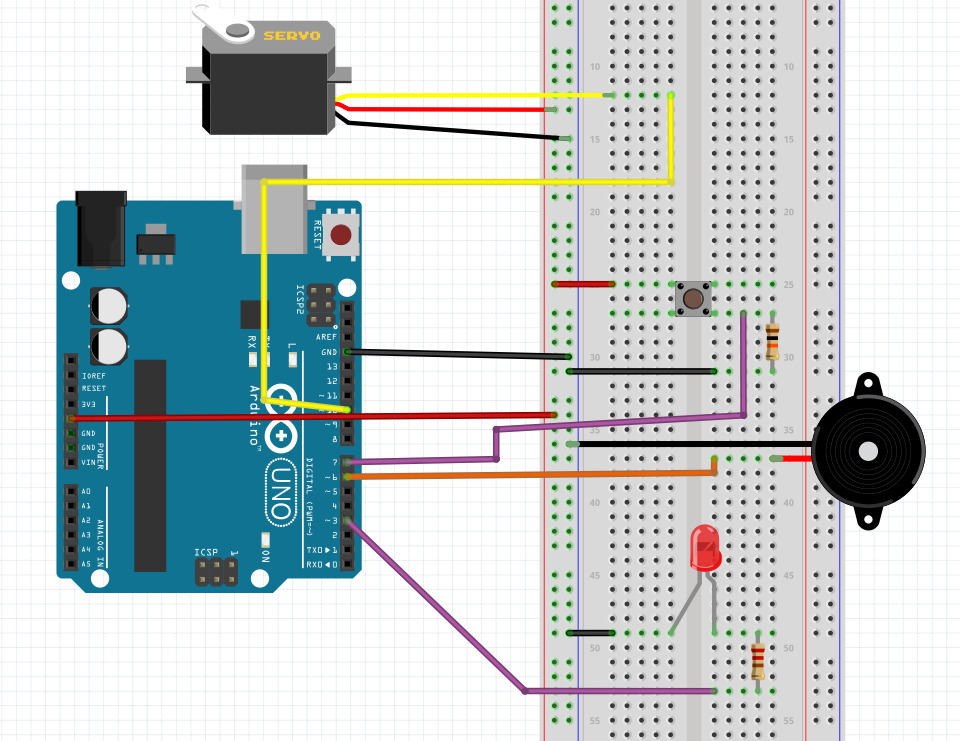
\includegraphics[height=5cm]{img/07.jpg}
\end{center}

\subsection{Pasos para desarrollar el proyecto}
\begin{enumerate}
	\item Montar un botón en el puerto 7 y un servomotor en el puerto 10 (HW)
	\item El servomotor debe hacer oscilar su brazo a intervalos de 1 segundo entre sus dos
		extremos solo si el botón se pulsa, el servomotor se detendrá si el botón se suelta (SW)
	\item Montar un LED rojo en el puerto 3 que debe encenderse si el botón del puerto 7 NO está
		pulsado (HW + SW)
	\item Añadir un piezoeléctrico al puerto 6 que sonará cuando el botón NO ESTÉ PULSADO (HW + SW)
\end{enumerate}

\begin{listing}[H]
\begin{minted}[linenos=true,bgcolor=bg,autogobble]{c++}
#include <Servo.h>

Servo s;

void setup() {
  pinMode(3, OUTPUT);  // LED
  pinMode(6, OUTPUT);  // Piezoeléctrico
  pinMode(7, INPUT);   // Botón
  s.attach(10);        // Servomotor
}

void loop() {
  if (digitalRead(7)==HIGH){ // Botón pulsado
    digitalWrite(3, LOW);
    s.write(10);
    delay(1000);
    s.write(170);
    delay(1000);
  } else {                   // Botón NO pulsado
	digitalWrite(3, HIGH);
	tone(6, 4000, 2000);
	delay(2000);
  }
}
\end{minted}
	\caption{Segundo software del proyecto \thesection}
\end{listing}

\newpage
%--------------------------------------------------------------------------
\section{Resistencia variable (potenciómetro)}

\begin{center}
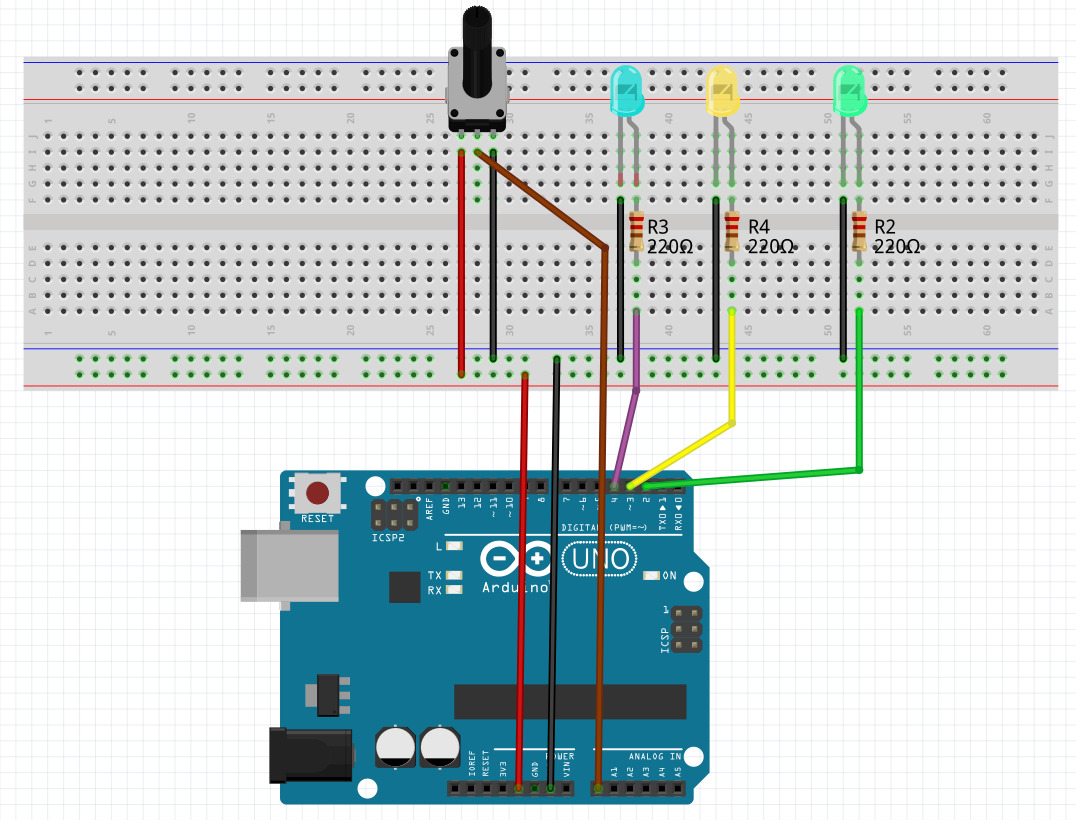
\includegraphics[height=5cm]{img/08.jpg}
\end{center}

\textbf{Este proyecto no se firma} Este es un proyecto que servirá para realizar pruebas.

\subsection{Pasos para desarrollar el proyecto}
\begin{enumerate}
	\item Montar la resistencia variable siguiendo los pasos indicados
	\item Montar los tres LED sobre la placa
	\item Escribir el software
	\item Modificar el software para que las luces funcionen al revés
\end{enumerate}

\begin{listing}[H]
\begin{minted}[linenos=true,bgcolor=bg,autogobble]{c++}

int x = 0;             // Variable

void setup() {
  pinMode(2, OUTPUT);  // LED
  pinMode(3, OUTPUT);  // LED
  pinMode(4, OUTPUT);  // LED
  Serial.begin(9600);  // Monitor serie
}

void loop() {
	x = analogRead(A0);
	Serial.println(x);
	if (x <= 200) {
		digitalWrite(2, HIGH);
		digitalWrite(3, LOW);
		digitalWrite(4, LOW);
	}
	if (x > 200 && x < 400) {
		digitalWrite(2, LOW);
		digitalWrite(3, HIGH);
		digitalWrite(4, LOW);
	}
	if (x >= 400) {
		digitalWrite(2, LOW);
		digitalWrite(3, LOW);
		digitalWrite(4, HIGH);
	}
}
\end{minted}
	\caption{Segundo software del proyecto \thesection}
\end{listing}

\newpage
%--------------------------------------------------------------------------
\section{Pitidos de frecuencia variable}

\subsection{Pasos para desarrollar el proyecto}
\begin{enumerate}
	\item Montar la resistencia variable (potenciómetro) de manera que su salida se encuentre conectada con el
		puerto analógico A0 y un piezoeléctrico en el puerto 9. También es necesario montar un LED
		de color rojo en el puerto 7 y otro de color verde en el puerto 8. [HW]
	\item Escribir el software que permita mostrar en la pantalla del ordenador mediante el monitor
		serie el valor de la resitencia variable (potenciómetro). [SW]
	\item Hacer que el piezoeléctrico emita pitidos con intervalos de un segundo entre un pitido y
		el siguiente. La frecuencia del pitido estará dado por el valor indicado en el
		potenciómetro según la fórmula $f=2*x+500$, donde $f$ es la frecuencia del pitido y $x$ es el
		valor del potenciómetro. Mientras se emite un pitido el LED rojo estará encendido y se
		apagará cuando deje de sonar el pitido. [SW]
	\item Hacer que el pitido siempre se emita a 2000 hercios pero el intervalo de espera entre un
		pitido y el siguiente sea variable en función de la posición del potenciómetro. Además el
		LED verde se encenderá cuando el piezo eléctrico no emita sonido. [SW]
\end{enumerate}


\newpage
%--------------------------------------------------------------------------
\section{Batería musical}

\subsection{Pasos para desarrollar el proyecto}
\begin{enumerate}
	\item Conecta el servomotor al puerto 10 y comprobar que se mueve [HW + SW]
	\item Construye una estructura con envases de plástico o de metal [HW]
	\item Consigue que la máqina sea capaz de hacer un ritmo sencillo, es decir, un golpe en
		cada uno de los envasas y a continuación un golpe en el otro envase [SW]
	\item Logra que la máquina realice un ritmo complejo, es decir, además de alternar golpes entre los
		dos envases, en alguno de ellos debe ser capaz de dar dos o más golpes seguidos [SW]
\end{enumerate}

\newpage
%--------------------------------------------------------------------------
\section{Servo y joystick coordinados}

\subsection{Pasos para desarrollar el proyecto}
\begin{enumerate}
	\item Poner un joystick conectado al puerto A1 y un servomotor en el puerto 9 [HW]
	\item Mostrar en el monitor serie el valor tomado por la entrada analógica y ver como varía
		según mueves el mando en el eje X [SW]
	\item Poner un servomotor que gire y adopte un ángulo proporcional a la entrada analógica del 
		anterior apartado: `s1.write(analogRead(A1)/6.5);` [HW y SW]
	\item Un LED rojo se encenderá solo si el servomotor se encuentra cerca de uno de sus límites de
		movimiento [SW]
\end{enumerate}

%--------------------------------------------------------------------------
\section{Servo y joystick con luces}

\subsection{Pasos para desarrollar el proyecto}
\begin{enumerate}
	\item El servomotor se mueve en función del movimiento del joystick [HW y SW]
	\item Cuando el servomotor se mueve a un lado se enciende una luz roja [HW y SW]
	\item Cuando el servomotor se mueve al otro lado se encuende la luz verde [HW y SW]
	\item Cuando el servomotor está en el centro las luces deben parpadear [SW]
\end{enumerate}


%--------------------------------------------------------------------------
\section{Piano de tres botones}

\subsection{Pasos para desarrollar el proyecto}
\begin{enumerate}
	\item Poner botón en el puerto 4 y piezoeléctrico en el puerto 9 [HW]
	\item Si se pulsa el botón debe sonar una nota musical f=261.63 Hz y duración t=250
		milisegundos. [SW]  \\

		Recuerda como se usaba tone con estos ejemplos: \\


\begin{listing}[H]
\begin{minted}[linenos=true,bgcolor=bg,autogobble]{c++}
void setup(){
    pinMode(9, OUTPUT);
}

void loop(){
    //tone(PUERTO,FRECUENCIA,TIEMPO);
    tone(9,        3000.0,     1000);
}
\end{minted}
	\caption{Segundo software del proyecto \thesection}
\end{listing}

	\item Añadir dos botones más en los puertos 5 y 6 [HW]
	\item Al pulsar los botones 5 y 6 deben sonar las notas musicales con frecuencias f=293.66 Hz y
		f=329.63 Hz [SW]
\end{enumerate}




%--------------------------------------------------------------------------
\section{Sensor de distancia}

\begin{center}
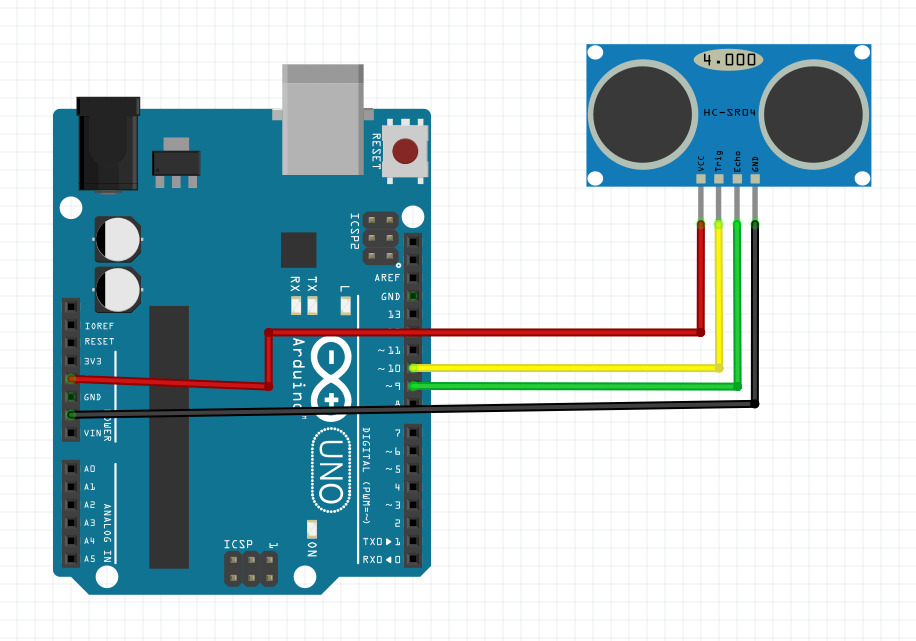
\includegraphics[height=6cm]{img/09.jpg}
\end{center}

\begin{listing}[H]
\begin{minted}[linenos=true,bgcolor=bg,autogobble]{c++}
// PRIMER SOFTWARE -----------------------------------
long t;    // Tiempo
long x;    // Espacio o distancia

void setup(){
    pinMode(10, OUTPUT);  // Disparador
    pinMode(9, INPUT);    // Receptor
}

void loop(){
    delayMicroseconds(2);
	digitalWrite(10, HIGH);
    delayMicroseconds(10);
    digitalWrite(10, LOW);
	t = pulseIn(9, HIGH);
	x = t * 0.017;
}
\end{minted}
	\caption{Primer software del proyecto \thesection}
\end{listing}


\begin{listing}[H]
\begin{minted}[linenos=true,bgcolor=bg,autogobble]{c++}
// SEGUNDO SOFTWARE ------------------------------------
void setup(){
    Serial.begin(9600);
}

void loop(){
    Serial.println(x);
}
\end{minted}
	\caption{Segundo software del proyecto \thesection}
\end{listing}

\subsection{Pasos para desarrollar el proyecto}
\begin{enumerate}
	\item Conectar el cableado siguiendo el esquema [HW]
	\item Escribir el primer software[SW]
	\item Añadir al primer software el segundo [SW]
    \item Modificarlo para que ponga en el monitor serie un mensaje cuando el sensor detecte corta
		distancia
\end{enumerate}


%--------------------------------------------------------------------------
\section{Sensor de distancia avanzado}

\subsection{Pasos para desarrollar el proyecto}
\begin{enumerate}
	\item Implementar el diseño de hardware del proyecto anterior [HW]
	\item Añadir dos luces LED, una roja y una verde [HW]
	\item Programa el software que permita que la luz verde se encienda si el objeto está lejos y la
		roja si el objeto que detecta el sensor está cerca [SW]
    \item Añade un piezoeléctrico que debe pitar en caso de que el objeto que detecta el sensor está
		extremadamente cerca [SW+HW]
\end{enumerate}
%## Proyecto 1: Sensor de luz y LED RGB

%1. Poner un LED RGB en la placa en los puertos 9, 10 y 11,
%	patas de larga a corta: GND, Verde, Azul, Rojo
%2. Añadir un sensor fotoresistencia que funcionará como 
%	un botón en el puerto A0
%3. Si la cantidad de luz medida es mayor a 700 el LED RGB
%	se encenderá en color verde, en caso contrario, en
%	color rojo
%4. Si la cantidad de luz recibida por la fotorresistencia
%es inferior a 100, el LED RGB se encenderá en color 
%	blanco
%--------------------------------------------------------------------------
%\section{Luces controladas por sensor de distancia}
%\subsection{Pasos para desarrollar el proyecto}
%\begin{enumerate}
%	\item Pon dos LEDs de diferentes colores en los puertos 3 y 4 y un sensor de distancia en 12 y 13
%	\item Escribir el software que muestre en pantalla el valor numérico de la distancia a un obstáculo
%	\item Según la distancia del sensor al obstáculo deben encenderse una luz, dos o ninguna
%	\item Un piezoeléctrico emitirá un pitido en caso de que el obstáculo esté demasiado cerca
%\end{enumerate} 



%## Proyecto 4: Portero controlado por mando analógico
%
%1. Conecta el joystick analógico al puerto A1 y el 
%	servomotor al puerto 9
%2. Escribe el software que mueve el servomotor a 
%	izquierda  y derecha en función del movimiento del 
%	joystick
%3. Construye la portería y el portero que deben 
%	sostenerse por sí mismos en pie
%4. Un piezoeléctrico emitirá un pitido SI SE PULSA
%	un botón (añadir piezoeléctrico y botón)





%\subsection{Pasos para desarrollar el proyecto}
%\begin{enumerate}
%	\item Conectar un joystick en el puerto A1 y un servomotor en el puerto 9
%	\item Mostrar en el monitor serie el valor tomado por la entrada analógica y ver como varía
%		según mueves el mando en el eje X
%	\item Poner un servomotor que guire y adopte un ángulo proporcional a la entrada analógica del
%		anterior apartado `s.write(analogRead(A1)/6.5);`
%	\item Un LED rojo debe encenderse cuando la posición del joystick se encuentre cerca de los
%		límites del movimiento
%\end{enumerate}
%
%\begin{listing}[H]
%\begin{minted}[linenos=true,bgcolor=bg,autogobble]{c++}
%#include <Servo.h>
%
%Servo s;
%
%void setup() {
%  pinMode(3, OUTPUT);  // LED
%  pinMode(6, OUTPUT);  // Piezoeléctrico
%  pinMode(7, INPUT);   // Botón
%  s.attach(10);        // Servomotor
%}
%
%void loop() {
%  if (digitalRead(7)==HIGH){ // Botón pulsado
%    digitalWrite(3, LOW);
%    s.write(10);
%    delay(1000);
%    s.write(170);
%    delay(1000);
%  } else {                   // Botón NO pulsado
%	digitalWrite(3, HIGH);
%	tone(6, 4000, 2000);
%	delay(2000);
%  }
%}
%\end{minted}
%	\caption{Segundo software del proyecto \thesection}
%\end{listing}



%\pagebreak
%
%# Segunda evaluación
%
%
%
%
%	
%
%
%## Proyecto 4: Portero controlado por mando analógico
%
%1. Conecta el joystick analógico al puerto A1 y el 
%	servomotor al puerto 9
%2. Escribe el software que mueve el servomotor a 
%	izquierda  y derecha en función del movimiento del 
%	joystick
%3. Construye la portería y el portero que deben 
%	sostenerse por sí mismos en pie
%4. Un piezoeléctrico emitirá un pitido SI SE PULSA
%	un botón (añadir piezoeléctrico y botón)
%	
%# Tercera evaluación
%
%## Proyecto 2: Piano de tres botones
%1. Poner botón en el puerto 4 y piezoeléctrico en el 
%	puerto 9
%2. Si se pulsa el botón debe sonar una nota musical 
%	f=261.63 Hz y duración 250 milisegundos
%	Recuerda: `tone(puerto, frecuencia, duración);` 
%3. Añadir dos botones más en los puertos 5 y 6
%4. Al pulsar los botones 5 y 6 deben sonar las notas
%	musicales con frecuencias f=293.66 Hz y 
%	f=329.63 Hz


\end{document}
